% Copyright (C) Data Structures and Algorithms Team.
\chapter{Heap}
A heap can be thought of as a simple tree data structure, however a heap usually employs one of two strategies:

\begin{enumerate}
\item min heap
\item max heap
\end{enumerate}

Each strategy determines the properties of the tree and it's values, e.g. if you were to choose the strategy min heap then each parent node would have a value that is $\leq$ than it's children, thus the node at the root of the tree will have the smallest value in the tree, the opposite is true if you were to use max heap. Generally as a rule you should always assume that a heap employs the min heap strategy unless otherwise stated.

Unlike other tree data structures like the one in \S\ref{bst} a heap is generally implemented as an array rather than a series of nodes who each have references to other nodes, both however contain nodes that have at most two children. Figure \ref{fig:tree_array_representation} shows how the tree (not a heap data structure) ($12~7$($3~2$)~$6$($9$~~)) would be represented as an array.

\begin{figure}
\begin{center}
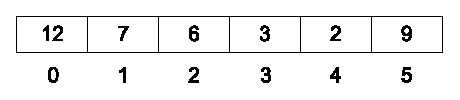
\includegraphics{heap_tree_array_representation}
\end{center}
\caption{Array representation of a simple tree data structure} \label{fig:tree_array_representation}
\end{figure}

Because we are using an array we need some way to calculate the index of a parent node, and the children of a node this is very simple, the expressions are defined below:

\begin{enumerate}
\item ($index - 1$)/$2$ (parent index)
\item $2 * index + 1$ (left child)
\item $2 * index + 2$ (right child)
\end{enumerate}

In Figure \ref{fig:heap_tree_array_representation_indexes} a) represents the calculation of the right child of $12$ ($2 * 0 + 2$); and b) calculates the index of the parent of $3$ (($3 - 1$)/$2$).

\begin{figure}
\begin{center}
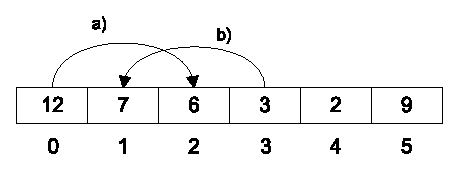
\includegraphics{heap_tree_array_representation_indexes}
\caption{Calculating node properties} \label{fig:heap_tree_array_representation_indexes}
\end{center}
\end{figure} 


